% preamble and style file for M&R lecture slides
\documentclass[11.5pt,sans,english]{beamer}

\usetheme{EastLansing}
\usecolortheme{lily}

\usepackage[most]{tcolorbox}

\usepackage{verbatim}
%\usepackage{ulem}
%\usepackage{fontawesome}
%\usepackage{tikz}
%\usepackage{pifont}
%\usepackage{tabularx}
\usepackage{array,booktabs,xcolor,colortbl,multirow,rotating,amssymb}
%\usepackage{amsmath}
% \usepackage{vwcol}
% \usepackage[T1]{fontenc}

  
\newcommand\vect[1]{\underline{\mathbf{#1}}}
\newcommand\unitvect[1]{\hat{\boldsymbol{#1}}}
%\newcommand\hatdot[1] { \hat{ \dot{ \boldsymbol{#1} } } }

\newtcbox
{\keyc}{on line,arc=2pt, colback=yellow!30!white, colframe=yellow!30!black, before upper={\rule[-3pt]{0pt}{10pt} },boxrule=1pt,boxsep=0pt,left=6pt,right=6pt,top=2pt,bottom=2pt,}

\newtcbox
{\keyb}{on line,arc=1pt, colback=blue!30!white, colframe=blue!30!black, before upper={\rule[-3pt]{0pt}{10pt} },boxrule=1pt,boxsep=0pt,left=6pt,right=6pt,top=2pt,bottom=2pt,}

\newtcbox
{\keyl}{on line,arc=1pt, colback=pink!30!white, colframe=blue!30!black, before upper={\rule[-3pt]{0pt}{10pt} },boxrule=1pt,boxsep=0pt,left=6pt,right=6pt,top=2pt,bottom=2pt,}

\newtcbox
{\keyw}{on line,arc=1pt, colback=red!30!white, colframe=blue!30!black, before upper={\rule[-3pt]{0pt}{10pt} },boxrule=1pt,boxsep=0pt,left=6pt,right=6pt,top=2pt,bottom=2pt,}

\newtcbox
{\keya}{on line,arc=1pt, colback=purple!30!white, colframe=blue!30!black, before upper={\rule[-3pt]{0pt}{10pt} },boxrule=1pt,boxsep=0pt,left=6pt,right=6pt,top=2pt,bottom=2pt,}

\newtcbox[auto counter,number within=section]
{keyf}
{
enhanced,
on line,
  boxsep=0pt,
  left=6pt,right=6pt,top=2pt,bottom=2pt,
  arc=5pt,
  boxrule=1pt,
  rightrule=38pt,
colback=green!10!white, 
colframe=green!50!black, 
title=\thetcbcounter,
detach title,
overlay unbroken and first ={
    \node[%rotate=90,
          %minimum width=1cm,
          anchor=south,
          font=\sffamily\bfseries\tiny,
          %yshift=-10pt,
          yshift=-5pt,
          xshift=-20pt,
          white]
    at (frame.east) {\thetcbcounter};
  }
}


\usepackage{xcolor}

%\usepackage{hyperref}
%\hypersetup{
%  pdfauthor={Lily Asquith},
%  urlcolor=blue,
%  colorlinks=true,
%  linkcolor=blue,
%  bookmarks=true
%}

%---------------------------------------------%
%              LILY'S COLOURS           %
%---------------------------------------------%
\definecolor{Wash}{RGB}{204,204,204}
%\definecolor{Pinky}{RGB}{254,200,254}%violet
\definecolor{Pinky}{RGB}{219,	240,	253}%violet
\definecolor{Bluey}{RGB}{0,190,255}%deep sky blue
\definecolor{DarkGrey}{RGB}{28,66,137}%dar grey
\definecolor{SussexWhite}{RGB}{253,255,254}%dar grey
\definecolor{LightGray}{RGB}{184,184,255}
\definecolor{YesGreen}{RGB}{0,128,0}
\definecolor{NoRed}{RGB}{250,0,0}



\definecolor{myred}{RGB}{255,153,153}
\definecolor{myorange}{RGB}{255,204,153}
\definecolor{myyellow}{RGB}{255,255,153}
\definecolor{mygreen}{RGB}{153,255,153}
\definecolor{mycyan}{RGB}{153,255,255}
\definecolor{myblue}{RGB}{153,204,255}
\definecolor{myviolet}{RGB}{153,153,255}
\definecolor{mypurple}{RGB}{204,153,255}
\definecolor{mypink}{RGB}{255,204,255}
\definecolor{mycoral}{RGB}{255,153,204}

%-----------------------------------------------------%
%              LILY'S COLUMN TYPES          %
%-----------------------------------------------------%
\newcolumntype{a}{>{\raggedright\arraybackslash}l}	
\newcolumntype{q}{>{\raggedright\arraybackslash}m{8cm}} 

%--------------------------------------------%
%              LILY'S SYMBOLS          %
%--------------------------------------------%
\newcommand{\dfinger}{\large{\textcolor{black}{\ding{43}}}\scriptsize}
\newcommand{\dstar}{\large{\textcolor{black}{\ding{76}}}\scriptsize}
\newcommand{\dwrite}{\large{\textcolor{black}{\ding{45}}}\scriptsize}
\newcommand{\ddiamond}{\small{\textcolor{DarkGrey}{\ding{117}}}\scriptsize}
\newcommand{\ddiamondwhite}{\small{\textcolor{SussexWhite}{\ding{117}}}\scriptsize}
\newcommand{\experiment}{\small{\textcolor{magenta}{\faCogs }}\scriptsize}
\newcommand{\watchit}{\textcolor{blue}{ \faYoutube}}


\makeatletter
\newcommand\notsotiny{\@setfontsize\notsotiny{6.5}{7.5}}
\makeatother


% 
\title[ Mechanics \& Relativity]{Mechanics \& Relativity}
%\subtitle{\textbf{Topic 1: Kinematics }}
\author[Dr Lily Asquith (Lily)]{ Dr Lily Asquith (Lily)}
\date[Week 2]{Week 2}
\logo{

\includegraphics[width=1.5cm]{../../utils/uslogo.jpg}
}


\begin{document}


\begin{frame}
\titlepage
\end{frame} 


\begin{frame}
\frametitle{Submit your workshop problem for marking by noon Friday}
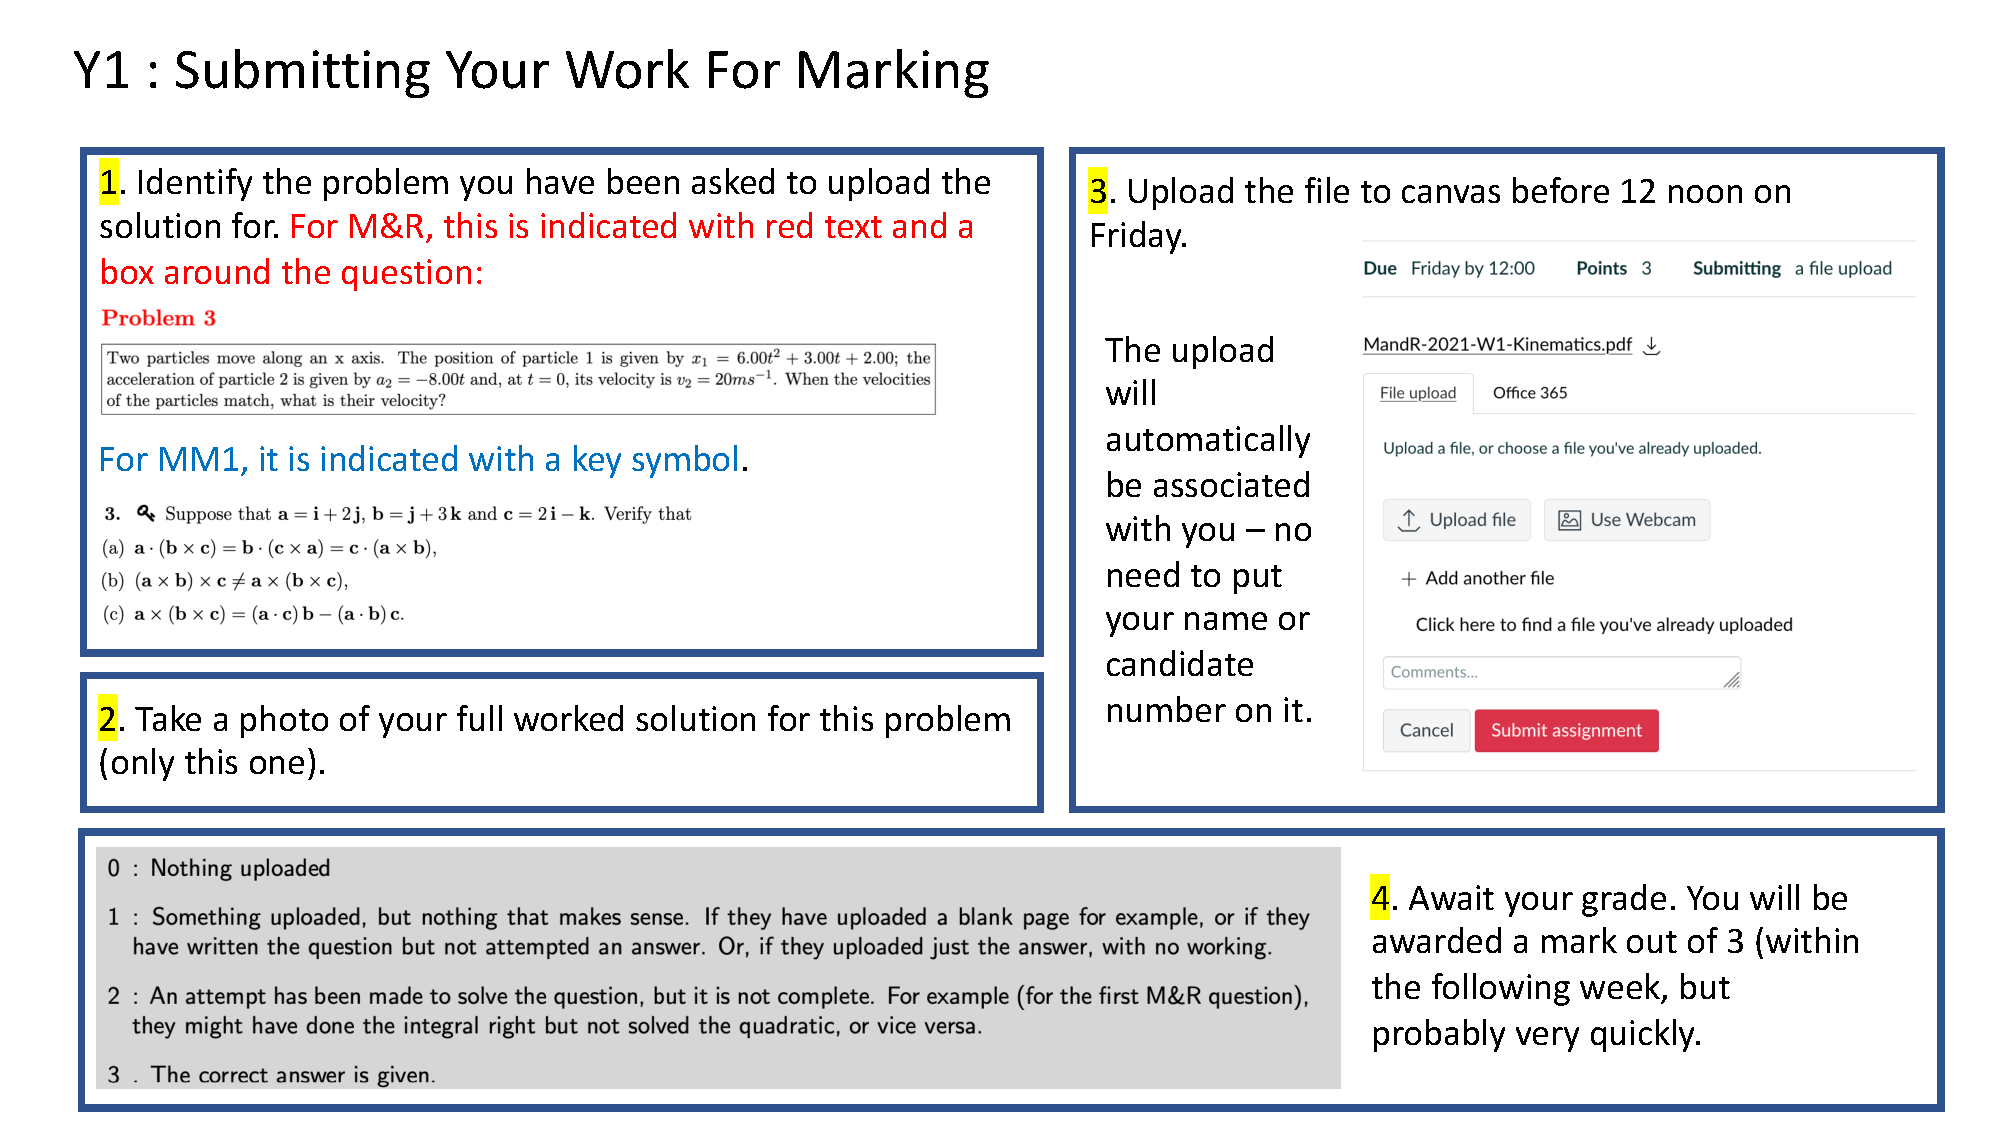
\includegraphics[scale=0.34]{Y1-2021-submission-guide.pdf}
The workshop problems (1 per week for 10 weeks) = 10\% of your final mark\\[1ex]
\end{frame} 

\begin{frame}
\frametitle{Adaptive practice}
There are three adaptive practice assignments for this week: 2.1, 2.2, 2.3.\\[1ex]
The adaptive practice quizzes (3 per week for 11 weeks) = 10\% of your final mark.\\[1ex]
But more importantly, they are exactly what you need to do to get a grasp of the topics covered in this module.\\[1ex]
\textbf{The reason for this module is to prepare you for what is next.}\\

\end{frame} 


 

 %-----------------------------------------------------------%
 % 1 Kinematics                                                 %
 %-----------------------------------------------------------%
\section{M\&R 2: Vectors for Physics}
\begin{frame}
\frametitle{Vectors} 
\normalsize

This week's topics:\\[3ex]

\begin{itemize}
\item[1.1] Intro to vectors for physics\\[3ex]
\item[1.2] Addition\\[3ex]
\item[1.3] Multiplication\\[3ex]
\end{itemize}
\end{frame} 
 
 \begin{frame}
\frametitle{Key formulae for the toilet door}

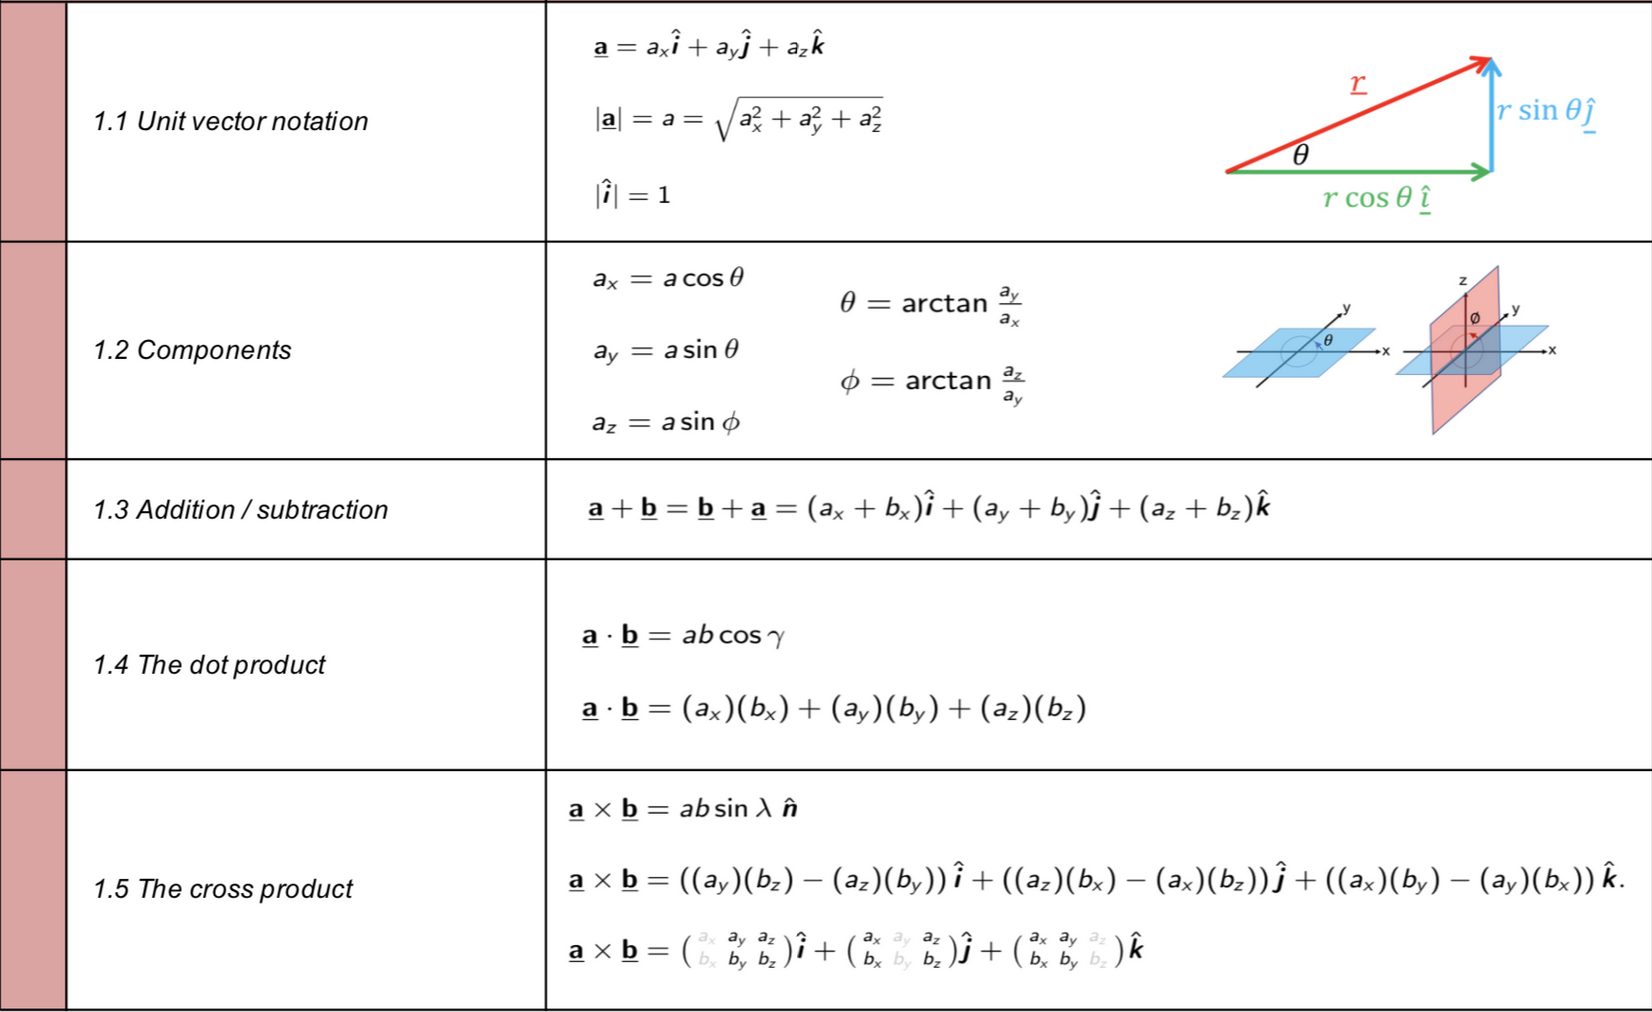
\includegraphics[scale=0.34]{keyf-vectors}
\end{frame}

 \subsection{Intro to vectors}

\begin{frame}{Why Vectors?}
\small

\includegraphics[scale=0.2]{descartes}

\end{frame}

\begin{frame}{The components of a vector}
\small

\end{frame}


\begin{frame}{The components of a vector}
\small

\end{frame}


\begin{frame}{A pinch of trigonometry}
\small

\end{frame}

\begin{frame}{Which way is up?}
\small

\end{frame}

\begin{frame}{Unit vector notation}
\small

\end{frame}

\begin{frame}{Worked example 1 (Ch 3 problem 1)}
\small
What are (a) the x component and (b) the y component of a vector in the xy plane if its direction is 250$^{\circ}$ counterclockwise from the positive direction of the x axis and its magnitude is 7.3 m?\\[20ex]

\end{frame}

\begin{frame}{Worked example 2 (Ch 3 problem 7)}
\small
 Consider two displacements, one of magnitude 3 m and another of magnitude 4 m. Show how the displacement vectors may be combined to get a resultant displacement of magnitude (a) 7 m, (b) 1 m, and (c) 5 m.\\[20ex]

\end{frame}


% LEC 2

 \subsection{Addition \& Subtraction} %1.4
 
 
\begin{frame}{Adding vectors}
\small

\end{frame}


 \begin{frame}{Worked example 3}
\small
Two vectors are given:\\[2ex]
What is $\vect{a} + \vect{b}$? \\[2ex]
What is $\vect{a} - \vect{b}$? \\[2ex]
What is the magnitude of ($\vect{a} + \vect{b}$)? \\[2ex]
What is the angle of $\vect{a}$ wrt the positive $\unitvect{i}$ direction?\\[2ex]
What is the angle between $\vect{a}$ and $\vect{b}$?\\[2ex]
\end{frame}

 \subsection{Multiplying vectors} %1.4
 
  \begin{frame}{The dot product}
\small

\end{frame}


  \begin{frame}{Worked Example 4 (Ch 3 problem 39) }
\small
Vector $\vect{a}$ has a magnitude of 6.00 units, vector $\vect{b}$ has a magnitude of 7.00 units, and $\vect{a} \cdot\vect{b} $ has a value of 14.0. What is the angle between the directions of $\vect{a}$ and $\vect{b} $ ?\\[20ex]


\end{frame}

  \begin{frame}{The cross product : spanner example}
\small

\end{frame}

  \begin{frame}{The cross product : graphically }
\small

\end{frame}

  \begin{frame}{The cross product : Lily's cartoon matrices }
\small

\end{frame}

% LEC 3

  \begin{frame}{Recap soh-cah-toa}
\small

\end{frame}



  \begin{frame}{Recap unit vector notation, components}
\small

\end{frame}

  \begin{frame}{Recap vector multiplication}
\small

\end{frame}

  \begin{frame}{Problem solving tools}
\small

\end{frame}

  \begin{frame}{Problem 1: What makes sense?}
\small
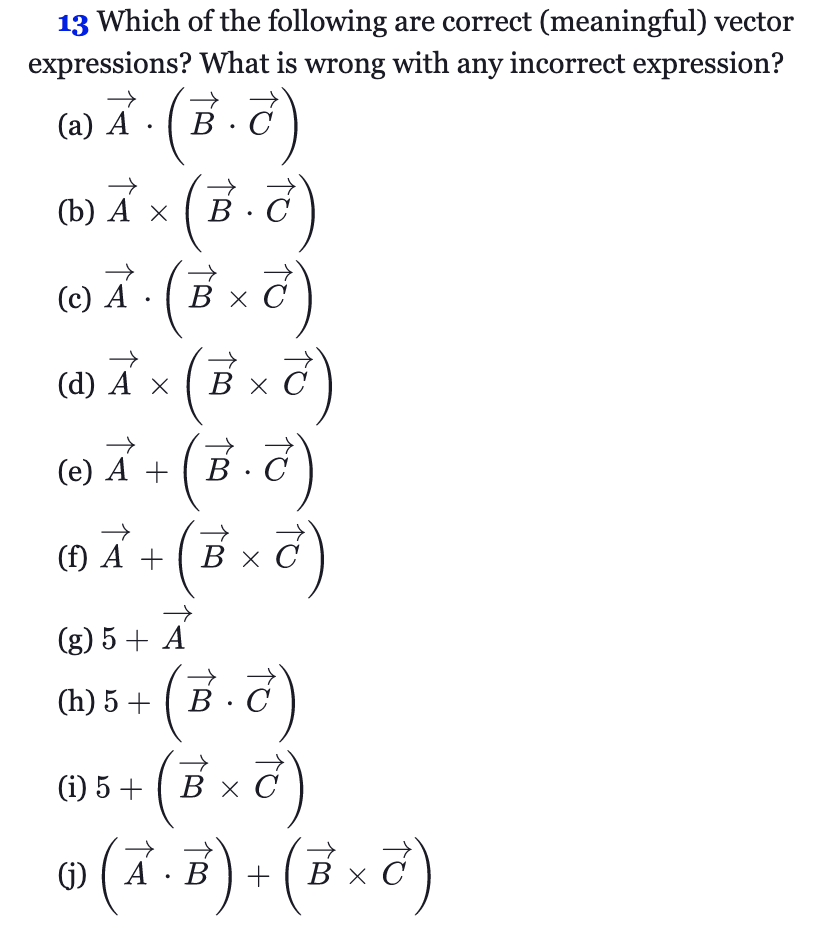
\includegraphics[scale=0.34]{whichmakesense}
\end{frame}

  \begin{frame}{Problem 2: The Dreaded Cube}
\small
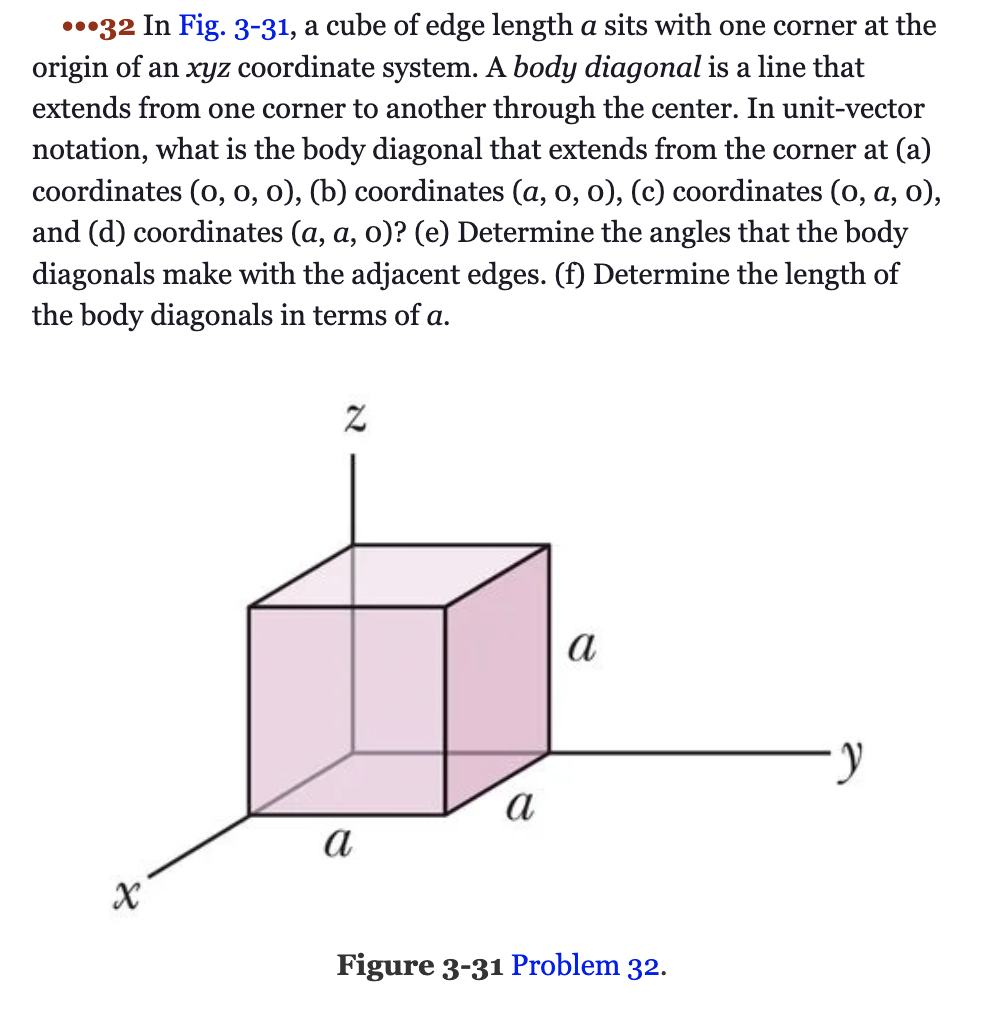
\includegraphics[scale=0.34]{dreadedcube}
\end{frame}



  \begin{frame}{Problem 3: Messing with the coordinates}
\small
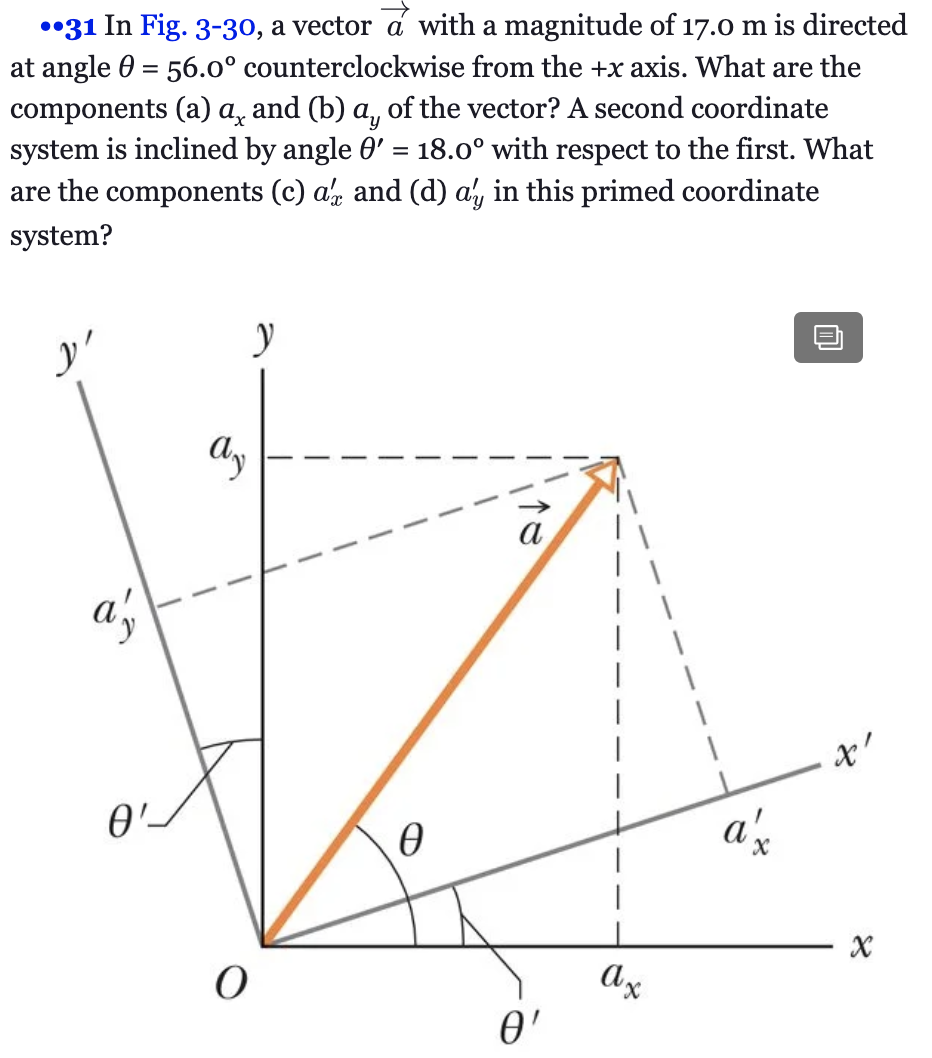
\includegraphics[scale=0.34]{coords}
\end{frame}

  \begin{frame}{Problem 4: The `Furious Product'}
\small
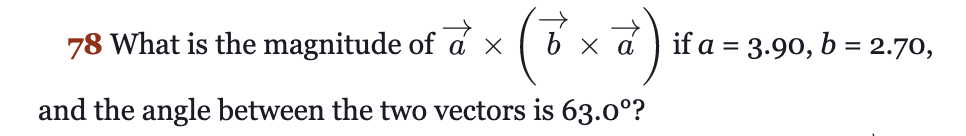
\includegraphics[scale=0.5]{furious}\\[18ex]

\end{frame}
%\begin{frame}{Before next lecture}
%
%Retry the pre-lecture quiz 2.1, if you like.\\[2ex]
%Attempt the pre-lecture quiz for 2.2 \\[2ex]
%See you tomorrow morning for lecture 2.2\\
%
%\end{frame}



 
\end{document}